\chapter{وراثة الجمهرات والانتقاء الطبيعي}\label{ch:b2:population-genetics}

في سنة 1848 اصطيدت فراشة فلفلية سوداء قرب مانشستر؛ وبحلول 1895
كانت تسع عشرة فراشة من كل عشرين في المدينة سوداء، وبحلول 1970، إذ
زال السخام، عاد الشكل الفاتح. ولم تتغير الفراشات: بل تغيرت
نسب أليلين في جمهرة من الملايين، تحت
أعين الطيور، في بضعة عشرات من الأجيال. وقد رأى داروين أن
الانتقاء لا بد أن يغير الأنواع لكن لم تكن لديه وسيلة لعدّه؛
والعدّ هو \omterm{def:b2:population-genetics:frequencies}{وراثة الجمهرات}، وهو حساب هذا
الفصل. فهو يسأل كيف تسلك تواترات الأليلات حين لا يفعل فيها
شيء، ثم كم بسرعة يحركها الانتقاء \omterm{def:b2:genome-diversification:mutation}{والطفرة} والهجرة والصدفة
\omterm{prop:b2:population-genetics:inbreeding}{والتزاوج الداخلي} --- وينتهي إلى الصفات التي ليست
مورّثة واحدة بل مورّثات كثيرة، وهي معظم ما يراه الانتقاء
فعلًا.

\section{المجمع المورّثي في سكون}

\begin{definition}[الجمهرة والمجمع المورّثي والتواترات]\label{def:b2:population-genetics:frequencies}
\index{وراثة الجمهرات}\index{مجمع مورّثي}\index{تواتر أليلي}
\emph{الجمهرة} مجموعة أفراد من نوع واحد
يتزاوجون فيما بينهم؛ و\emph{مجمعها المورّثي} مجموعة أليلاتهم كلها.
ولموقع له أليلان $A$ و$a$ في جمهرة ثنائية الصيغة من
$N$ فرد، تكون \emph{التواترات الأليلية} $p = (2N_{AA} +
N_{Aa})/2N$ و$q = 1 - p$، وتكون \emph{تواترات الأنماط الوراثية}
كسور $AA$ و$Aa$ و$aa$. والتطور، بالمعنى الأضيق،
تغير في التواترات الأليلية بين جيلين؛
وسؤال هذا الفصل ما الذي يغيرها وبكم.
\end{definition}

\begin{theorem}[هاردي--واينبرغ]\label{thm:b2:population-genetics:hw}
\index{قانون هاردي--واينبرغ}
في جمهرة كبيرة تتزاوج عشوائيًا، بلا انتقاء ولا \omterm{def:b2:genome-diversification:mutation}{طفرة}
ولا هجرة، لا تتغير التواترات الأليلية من جيل
إلى الذي يليه، وبعد جيل واحد من التزاوج
العشوائي تكون تواترات الأنماط الوراثية
\[
AA : p^{2}, \qquad Aa : 2pq, \qquad aa : q^{2},
\]
وتبقى كذلك. والسيادة لا تجعل \omterm{def:b2:meiosis-heredity:vocabulary}{الأليل} \omterm{def:b2:meiosis-heredity:vocabulary}{السائد} ينتشر، ولا
يضيع \omterm{def:b2:meiosis-heredity:vocabulary}{الأليل} المتنحي النادر: بل يختبئ في متغايري اللواقح،
وهم يفوقون متماثلي اللواقح بنسبة $2p/q$ إلى واحد --- فعند $q = 0.01$
تكون النسبة مئتين إلى واحد. والقانون هو الفرضية الصفرية \omterm{def:b2:population-genetics:frequencies}{لوراثة
الجمهرات}: فالخروج عليه في جمهرة حقيقية، أو تغير
$p$ بين جيلين، توقيع إحدى القوى
التالية.
\end{theorem}
\begin{proof}
التزاوج العشوائي اتحاد عشوائي للأعراس: فالعرس يحمل $A$
باحتمال $p$ ويحمل $a$ باحتمال $q$، مستقلًا عن
شريكه، فتكون اللاقحة $AA$ باحتمال $p^{2}$، و$Aa$ باحتمال
$2pq$، و$aa$ باحتمال $q^{2}$. \omterm{def:b2:population-genetics:frequencies}{والتواتر الأليلي} في الجيل
التالي هو $p' = p^{2} + \tfrac12(2pq) = p(p + q) = p$: أي لم يتغير.
ولمّا كانت تواترات الأنماط الوراثية لا تتعلق إلا بالمقدار $p$، كانت هي نفسها
في كل جيل بعد الأول.
\end{proof}

\begin{example}[قراءة تواتر]\label{ex:b2:population-genetics:cf}
التليف الكيسي \omterm{def:b2:meiosis-heredity:vocabulary}{متنحٍّ}، ويصيب طفلًا أوروبيًا من كل 2500:
أي $q^{2} = 1/2500$، و$q = 0.02$، ويكون تواتر الحاملين $2pq
\approx 0.04$ --- فشخص من كل 25 يحمل أليلًا يقتل
متماثلي لواقحه، و\qty{98}{\%} من نسخ \omterm{def:b2:meiosis-heredity:vocabulary}{الأليل} تجلس في
حاملين أصحاء حيث لا يستطيع الانتقاء رؤيتها. وذلك سبب إزالة
المتنحي المميت ببطء شديد، وسبب أن مخططات تحسين النسل الرامية إلى
إفناء الأمراض المتنحية بتعقيم المصابين ما كان لها أن
تنجح أبدًا: فحساب القسم التالي يبيّن كم ذلك
بطيء.
\end{example}

\section{الانتقاء}

\begin{definition}[اللياقة]\label{def:b2:population-genetics:fitness}
\index{لياقة}\index{معامل الانتقاء}
\emph{لياقة} \omterm{def:b2:meiosis-heredity:vocabulary}{نمط وراثي} $w$ هي إسهامه النسبي
بالخلف في الجيل التالي --- أي البقاء إلى التكاثر
في الخصوبة، مقيسًا بحيث يكون لأفضل \omterm{def:b2:meiosis-heredity:vocabulary}{نمط وراثي} $w = 1$. و\emph{معامل
الانتقاء} $s$ \omterm{def:b2:meiosis-heredity:vocabulary}{لنمط وراثي} هو قصوره،
$w = 1 - s$. واللياقة خاصة \omterm{def:b2:meiosis-heredity:vocabulary}{لنمط وراثي} في بيئة،
لا \omterm{def:b2:meiosis-heredity:vocabulary}{لأليل} في ذاته: \omterm{def:b2:meiosis-heredity:vocabulary}{فأليل} الفراشة السوداء كان له $w > 1$
نسبةً إلى الفاتحة على لحاء مسخَّم و$w < 1$ على الأشنة.
\end{definition}

\begin{theorem}[الانتقاء يغير التواتر الأليلي]\label{thm:b2:population-genetics:selection}
\index{الانتقاء الطبيعي!معادلة}
عند لياقات أنماط وراثية $w_{AA}$ و$w_{Aa}$ و$w_{aa}$، تكون \omterm{def:b2:population-genetics:fitness}{اللياقة}
المتوسطة $\bar w = p^{2}w_{AA} + 2pq\,w_{Aa} + q^{2}w_{aa}$ ويكون
\omterm{def:b2:population-genetics:frequencies}{التواتر الأليلي} في الجيل التالي
\[
p' = \frac{p^{2}w_{AA} + pq\,w_{Aa}}{\bar w}, \qquad
\Delta p = p' - p = \frac{pq\,\bigl[p(w_{AA} - w_{Aa}) + q(w_{Aa} - w_{aa})\bigr]}{\bar w}.
\]
ولذلك نتيجتان. أولاهما أن $\Delta p$ يتناسب مع $pq$: فالانتقاء
أسرع ما يكون عند التواترات المتوسطة وأبطأ ما يكون حين يكون \omterm{def:b2:meiosis-heredity:vocabulary}{الأليل}
نادرًا أو شبه مثبَّت --- إذ لا يبقى تنوع كثير ليفعل فيه.
والثانية أنه ضد \omterm{def:b2:meiosis-heredity:vocabulary}{أليل} \omterm{def:b2:meiosis-heredity:vocabulary}{متنحٍّ} ($w_{AA} = w_{Aa} = 1$، و$w_{aa} =
1 - s$) يكون التغير $\Delta q = -s\,pq^{2}/\bar w$، متناسبًا
مع $q^{2}$: فالمتنحي النادر شبه خفي على الانتقاء،
وتنصيف تواتره من $0.01$ يستغرق نحو مئة جيل
حتى حين يكون متماثلو لواقحه مميتين. \omterm{def:b2:meiosis-heredity:vocabulary}{والأليل} \omterm{def:b2:meiosis-heredity:vocabulary}{السائد} المحبَّذ
ينتشر سريعًا في البداية ثم يتلكأ في النهاية، للسبب
نفسه.
\end{theorem}
\begin{proof}
من الخلف يكون كسر $p^{2}w_{AA}/\bar w$ من نمط $AA$ ويكون
$2pq\,w_{Aa}/\bar w$ من نمط $Aa$ (إذ يوزن تواتر كل \omterm{def:b2:meiosis-heredity:vocabulary}{نمط وراثي}
بلياقته ويُعاد تسويته)؛ وأليلات $A$ بينها هي كل
الأول ونصف الثاني، فيعطيان $p'$. وبطرح $p =
p\bar w/\bar w$ ونشر $\bar w$ نحصل على $\Delta p$. وفي حالة \omterm{def:b2:meiosis-heredity:vocabulary}{متنحٍّ}
مميت ($s = 1$): $q' = q^{2}\cdot 0 + pq$ مقسومًا على $\bar w = 1 -
q^{2}$، فيكون $q' = q/(1 + q)$، ومن ثم $1/q' = 1/q + 1$ وبعد $t$
جيلًا يكون $1/q_t = 1/q_0 + t$: فالانتقال من $q_0 = 0.01$ إلى $0.005$ يستغرق
$t = 100$.
\end{proof}

\begin{omfigure}
\begin{tikzpicture}
\begin{axis}[
  width=0.8\linewidth, height=6cm,
  axis x line=bottom, axis y line=left,
  xmin=0, xmax=150, ymin=0, ymax=1.05,
  xlabel={الأجيال}, ylabel={تواتر الأليل المحبَّذ},
  xlabel style={font=\small, at={(axis description cs:0.5,-0.11)}, anchor=north},
  ylabel style={font=\small},
  tick label style={font=\small}, xtick={0,50,100,150}, ytick={0,0.5,1},
  legend style={font=\scriptsize, at={(0.97,0.35)}, anchor=east, draw=none},
  clip=false,
]
\addplot[very thick, omDef] table[x=t, y=dom] {
t dom
0 0.01
10 0.02
20 0.04
30 0.075
40 0.14
50 0.24
60 0.38
70 0.53
80 0.66
90 0.76
100 0.83
110 0.88
120 0.91
130 0.93
140 0.945
150 0.955
};
\addlegendentry{الأليل المحبَّذ سائد، $s = 0.1$}
\addplot[very thick, omThm] table[x=t, y=rec] {
t rec
0 0.01
10 0.0101
20 0.0102
30 0.0104
40 0.0106
50 0.0108
60 0.011
70 0.0113
80 0.0116
90 0.012
100 0.0124
110 0.0128
120 0.0133
130 0.0138
140 0.0144
150 0.015
};
\addlegendentry{الأليل المحبَّذ متنحٍّ، $s = 0.1$}
\end{axis}
\end{tikzpicture}

{\small الانتقاء في العمل بأفضلية \qty{10}{\%}. \omterm{def:b2:meiosis-heredity:vocabulary}{فالأليل} \omterm{def:b2:meiosis-heredity:vocabulary}{السائد}
المحبَّذ يرتفع من \qty{1}{\%} إلى الأكثرية في سبعين
جيلًا ثم يبطئ، ومنافسه المتنحي النادر مختبئ في
متغايري اللواقح؛ أما \omterm{def:b2:meiosis-heredity:vocabulary}{الأليل} المتنحي المحبَّذ عند \qty{1}{\%} فلا يكاد
يتحرك في المدة نفسها، إذ لا يكاد يُكشف أبدًا.}
\end{omfigure}

\begin{proposition}[أصناف الانتقاء]\label{prop:b2:population-genetics:kinds}
\index{انتقاء موجّه}\index{انتقاء مثبِّت}\index{انتقاء موازن}\index{أفضلية متغاير اللواقح}
الانتقاء \emph{الموجّه} يحبّذ طرفًا واحدًا ويسوق
أليلًا نحو التثبيت (الفراشة السوداء في غابة مسخَّمة؛ ومقاومة
الصادات؛ وحجم منقار العصفور في جفاف).
والانتقاء \emph{المثبِّت} يحبّذ الوسط ويزيل
الأطراف (وزن ولادة الإنسان: فالأطفال الذين يموتون هم الأصغر
والأكبر)؛ وهو يبقي الجمهرة حيث هي وهو أشيع الأصناف.
والانتقاء \emph{المفرِّق} يحبّذ الطرفين
ضد الوسط، ويستطيع شق جمهرة
(\cref{ch:b2:speciation}). والانتقاء \emph{الموازن} يبقي
أليلين في الجمهرة إلى غير أجل: إما \emph{\omterm{prop:b2:population-genetics:kinds}{بأفضلية متغاير
اللواقح}}، حين يكون $Aa$ أليق من أي من متماثلي اللواقح --- فعند
$w_{AA} = 1 - s$ و$w_{aa} = 1 - t$ و$w_{Aa} = 1$، يستقر التواتر
عند $\hat p = t/(s + t)$ --- وإما بانتقاء \emph{متعلق بالتواتر}،
حين يكون \omterm{def:b2:meiosis-heredity:vocabulary}{النمط الوراثي} أليق كلما كان أندر (أليلات
$S$ النادرة في \cref{ch:b2:angiosperm-reproduction}، والفريسة التي لم
يتعلمها مفترس، وجهتا فم سمكة آكلة للحراشف).
\end{proposition}
\begin{proof}[شواهد]
خضاب الخلية المنجلية يقتل معظم متماثلي اللواقح قبل أن
يتكاثروا، ومع ذلك \omterm{def:b2:meiosis-heredity:vocabulary}{فالأليل} عند \qty{10}{\%} إلى \qty{20}{\%} في
أنحاء إفريقيا الملارية. وبيّن أليسون (1954) أن الأطفال متغايري اللواقح
كانت إصاباتهم الملارية أقل بكثير وأخف من أي من
متماثلي اللواقح، وأن تواتر \omterm{def:b2:meiosis-heredity:vocabulary}{الأليل} ينطبق على التوزع
التاريخي لملاريا المنجلية؛ وفي الجمهرات ذات الأصل
الإفريقي التي تعيش حيث لا ملاريا ما زال التواتر يهبط منذ ذلك الحين. وعند $t \approx 0.8$ \omterm{def:b2:meiosis-heredity:vocabulary}{لمتماثل اللواقح} المنجلي
و$s \approx 0.1$ \omterm{def:b2:meiosis-heredity:vocabulary}{لمتماثل اللواقح} السوي في منطقة ملارية،
يكون $\hat q = s/(s + t) \approx 0.11$ --- وهو ما يُلاحظ.
\end{proof}

\section{الطفرة والهجرة والتوازن}

\begin{theorem}[توازن الطفرة والانتقاء]\label{thm:b2:population-genetics:balance}
\index{توازن الطفرة والانتقاء}\index{حمل وراثي}
\omterm{def:b2:meiosis-heredity:vocabulary}{الأليل} الضار تغذيه \omterm{def:b2:genome-diversification:mutation}{الطفرة} بمعدل $\mu$ لكل عرس
في الجيل ويزيله الانتقاء. وعند التوازن يتعادل
الاثنان: فلأليل \omterm{def:b2:meiosis-heredity:vocabulary}{متنحٍّ} ضرره عند تماثل اللواقح $s$،
\[
\hat q = \sqrt{\mu/s}\,;
\]
ولأليل \omterm{def:b2:meiosis-heredity:vocabulary}{سائد} (أو \omterm{def:b2:meiosis-heredity:vocabulary}{سائد} جزئيًا) ضرره عند تغاير اللواقح
$hs$ يكون $\hat q = \mu/hs$. ومن ثم فالتواتر التوازني
\omterm{def:b2:meiosis-heredity:vocabulary}{لمتنحٍّ} كبير حتى لو كان مميتًا: فعند $\mu = 10^{-5}$ و
$s = 1$ يكون $\hat q = 3\times 10^{-3}$، ويحمله \qty{0.6}{\%} من الجمهرة.
وكل جمهرة تحمل \emph{حملًا وراثيًا} كهذا عند
آلاف المواقع، معظمه \omterm{def:b2:meiosis-heredity:vocabulary}{متنحٍّ} مختبئ، وتوازن
حجة السقّاطة في \cref{ch:b2:asexual-reproduction}
--- أي كسر $e^{-U/s}$ من الأفراد الخالين من الطفرات
الضارة --- هو التوازن نفسه مجموعًا على المورثوم.
\end{theorem}
\begin{proof}
في كل جيل تضيف \omterm{def:b2:genome-diversification:mutation}{الطفرة} $\mu p \approx \mu$ إلى $q$ ويزيل
الانتقاء $s\,pq^{2}/\bar w \approx sq^{2}$ (عند $q$ صغير)؛
ووضع $\mu = s\hat q^{2}$ يعطي نتيجة المتنحي. أما \omterm{def:b2:meiosis-heredity:vocabulary}{الأليل}
\omterm{def:b2:meiosis-heredity:vocabulary}{السائد} فيزيل الانتقاء منه $hs\,q$ في الجيل (إذ تُكشف كل نسخة
في متغاير لواقح)، فيكون $\mu = hs\hat q$.
\end{proof}

\begin{proposition}[الهجرة وقاعدة المهاجر الواحد]\label{prop:b2:population-genetics:migration}
\index{تدفق مورّثي}\index{هجرة (وراثية)}
إذا كان كسر $m$ من جمهرة في كل جيل مهاجرين وافدين
من جمهرة تواترها الأليلي $p_{m}$، تحرك التواتر
نحو $p_{m}$ بمقدار $\Delta p = m(p_{m} - p)$: فيخبو الفرق
بين الجمهرتين على صورة $(1 - m)^{t}$. \emph{\omterm{prop:b2:population-genetics:migration}{والتدفق
المورّثي}} يجانس؛ وهو ينقض \omterm{def:b2:plant-plasticity:plasticity}{التكيف} المحلي ما لم يكن الانتقاء
أقوى من $m$، وهو القوة التي تبقي النوع نوعًا
واحدًا. وبالمقابل فالجمهرات التي لا تتبادل مهاجرين تتباعد
بالانجراف وبطفراتها المنفصلة، ومهاجر واحد في
الجيل --- مهما كان حجم الجمهرة --- يكفي لمنعها
من الانجراف إلى تثبيت أليلات مختلفة.
\end{proposition}

\section{الصدفة: الانجراف الوراثي}

\begin{theorem}[الانجراف الوراثي]\label{thm:b2:population-genetics:drift}
\index{انجراف وراثي}\index{حجم فعّال للجمهرة}\index{تثبيت}
في جمهرة من $N$ فرد \omterm{def:b2:meiosis-heredity:meiosis}{ثنائي الصيغة}، يكون \omterm{def:b2:population-genetics:frequencies}{التواتر الأليلي} في كل
جيل عينة عشوائية من $2N$ عرسًا من
السابق، حتى يهيم $p$ عشوائيًا بتباين قدره
$p(1 - p)/2N$ في الجيل. و\emph{التغايُر اللاقحي} $H = 2pq$
يخبو وسطيًا بعامل $(1 - 1/2N)$ في كل جيل،
\[
H_t = H_0\left(1 - \frac{1}{2N}\right)^{t} \approx H_0\,e^{-t/2N},
\]
وينتهي كل \omterm{def:b2:meiosis-heredity:vocabulary}{أليل} إلى الضياع أو \emph{التثبيت}، باحتمال
يساوي تواتره الحالي: \omterm{def:b2:genome-diversification:mutation}{فالطفرة} المحايدة الجديدة،
عند تواتر $1/2N$، تُثبَّت باحتمال $1/2N$، وإن ثُبِّتت
استغرقت نحو $4N$ جيل لذلك. والانجراف مهمل في
جمهرة من الملايين وغالب في جمهرة من العشرات:
فحادث \emph{عنق الزجاجة} أو حادث \emph{التأسيس} --- بضعة مستعمرين على
جزيرة، أو نوع رُدّ إلى مئة فرد بالصيد --- يضيّع أليلات
بالصدفة في جيل واحد ويترك جمهرة متجانسة
فقيرة مليئة بمتماثلي اللواقح. و$N$ الذي يهم هو
الحجم \emph{الفعّال}، أي عدد الأفراد المتكاثرين فعلًا،
وهو عادةً أصغر بكثير من التعداد.
\end{theorem}
\begin{proof}
نسخ المورّثات $2N$ في الجيل التالي تُسحب مع الإعادة
من مجمع يكون فيه تواتر $A$ هو $p$: فعدد نسخ $A$
ثنائي الحد بمتوسط $2Np$ وتباين $2Np(1 - p)$، فيكون للمقدار $p'$
متوسط $p$ وتباين $p(1 - p)/2N$. ونسختان تُسحبان عشوائيًا في
الجيل التالي تأتيان من النسخة الأبوية نفسها باحتمال
$1/2N$ وتكونان حينئذ متطابقتين، فيُضرب احتمال اختلاف
نسختين (أي التغايُر اللاقحي) في $1 - 1/2N$ في كل
جيل. واحتمال التثبيت: تواتر \omterm{def:b2:meiosis-heredity:vocabulary}{الأليل} المحايد
مارتنغال --- فقيمته المنتظرة لا تتغير --- وينتهي عند 0
أو 1، فيكون احتمال انتهائه عند 1 مساويًا قيمته الابتدائية.
\end{proof}

\begin{omfigure}
\begin{tikzpicture}
\begin{axis}[
  width=0.82\linewidth, height=6cm,
  axis x line=bottom, axis y line=left,
  xmin=0, xmax=60, ymin=0, ymax=1.05,
  xlabel={الأجيال}, ylabel={التواتر الأليلي $p$},
  xlabel style={font=\small, at={(axis description cs:0.5,-0.11)}, anchor=north},
  ylabel style={font=\small},
  tick label style={font=\small}, xtick={0,20,40,60}, ytick={0,0.5,1},
  legend style={font=\scriptsize, at={(0.5,-0.25)}, anchor=north, draw=none, legend columns=2},
  clip=false,
]
\addplot[thick, omThm] coordinates {(0,0.5) (2,0.55) (4,0.62) (6,0.58) (8,0.7) (10,0.8) (12,0.75) (14,0.85) (16,0.92) (18,0.88) (20,0.95) (22,1) (60,1)};
\addlegendentry{$N = 10$}
\addplot[thick, omThm!60] coordinates {(0,0.5) (2,0.42) (4,0.35) (6,0.4) (8,0.3) (10,0.2) (12,0.25) (14,0.15) (16,0.1) (18,0.05) (20,0.08) (22,0.02) (24,0) (60,0)};
\addplot[thick, omDef] coordinates {(0,0.5) (5,0.52) (10,0.49) (15,0.53) (20,0.56) (25,0.54) (30,0.58) (35,0.55) (40,0.57) (45,0.6) (50,0.58) (55,0.61) (60,0.6)};
\addlegendentry{$N = 1000$}
\addplot[thick, omDef!60] coordinates {(0,0.5) (5,0.48) (10,0.5) (15,0.47) (20,0.45) (25,0.46) (30,0.44) (35,0.45) (40,0.43) (45,0.44) (50,0.42) (55,0.43) (60,0.42)};
\end{axis}
\end{tikzpicture}

{\small الانجراف. جمهرتان من عشرة أفراد تبدآن عند
$p = 0.5$ تثبتان أليلين متعاكسين في غضون خمسة وعشرين جيلًا؛ وجمهرتان
من ألف تهيمان ببضعة في المئة في ستين جيلًا.}
\end{omfigure}

\begin{proposition}[التزاوج الداخلي]\label{prop:b2:population-genetics:inbreeding}
\index{تزاوج داخلي}\index{معامل التزاوج الداخلي}\index{وهن التزاوج الداخلي}
التزاوج بين الأقارب لا يغير التواترات الأليلية لكنه
يرفع نسبة متماثلي اللواقح: أما \emph{\omterm{prop:b2:population-genetics:inbreeding}{معامل التزاوج الداخلي}}
$F$ لفرد فهو احتمال أن يكون أليلاه
عند موقع متطابقين بالنسب، وتصير تواترات الأنماط
الوراثية $p^{2} + Fpq$ و$2pq(1 - F)$ و$q^{2} + Fpq$. ولخلف
أبناء العم يكون $F = 1/16$، وللإخوة $1/4$، وللإلقاح
الذاتي $1/2$. ولمّا كانت الأليلات المتنحية \omterm{thm:b2:population-genetics:balance}{للحمل الوراثي}
تُكشف في متماثلي اللواقح الزائدين، عانى الخلف الداخلي
\emph{\omterm{prop:b2:population-genetics:inbreeding}{وهن التزاوج الداخلي}}: \omterm{def:b2:meiosis-heredity:vocabulary}{فمتنحٍّ} مميت عند $q = 0.01$
يظهر في $q^{2} = 10^{-4}$ من خلف التزاوج العشوائي لكنه يظهر في
$q^{2} + Fpq = 7\times 10^{-4}$ من أولاد أبناء العم، أي سبعة أضعاف؛
وبالجمع على آلاف المواقع، يكون لأولاد أبناء العم نحو
ضعفي وفيات الرضع عند غيرهم، وجمهرة صغيرة تتزاوج
داخليًا أجيالًا تفقد الخصوبة والعافية --- وهي محنة
الفهد والنمر الفلوريدي والبيوت المالكة في أوروبا.
\end{proposition}

\section{مورّثات كثيرة: الصفات الكمية}

\begin{theorem}[قابلية التوريث والاستجابة للانتقاء]\label{thm:b2:population-genetics:heritability}
\index{قابلية التوريث}\index{وراثة كمية}\index{معادلة المربّي}
الصفة كالطول أو المردود أو عمق المنقار تقررها مورّثات
كثيرة صغيرة الأثر وتقررها البيئة، وهي تتغير
تغيرًا متصلًا. وينقسم تباينها في جمهرة إلى جزء
\emph{وراثي} $V_G$ وجزء \emph{بيئي} $V_E$، وتكون
\emph{\omterm{thm:b2:population-genetics:heritability}{قابلية التوريث}} $h^{2} = V_A/V_P$ كسرَ التباين
الظاهري العائد إلى الآثار الجمعية للمورّثات (أي الجزء
المنقول). فإذا انتُقي آباء الجيل التالي
بمتوسط يفوق متوسط الجمهرة بمقدار $S$ (وهو
\emph{فرق الانتقاء})، فاق خلفهم المتوسط بمقدار
\[
R = h^{2}\,S
\]
--- وهي \emph{\omterm{thm:b2:population-genetics:heritability}{معادلة المربّي}}. وهي كل تربية الحيوان
والنبات في سطر واحد: فقابلية توريث قدرها $0.5$ وآباء أعلى من
المتوسط بانحراف معياري يعطون خلفًا أعلى منه بنصف انحراف
معياري، ويتراكم الكسب جيلًا بعد جيل.
\omterm{thm:b2:population-genetics:heritability}{وقابلية التوريث} خاصة لجمهرة في
بيئة، لا خاصة لصفة: فهي لا تقول شيئًا عما إذا كانت
الصفة ثابتة، والصفة التي لها $h^{2} = 0.8$ في جمهرة قد
يكون لها $h^{2} = 0$ في أخرى يملك فيها كل فرد \omterm{def:b2:meiosis-heredity:vocabulary}{النمط الوراثي}
نفسه.
\end{theorem}
\begin{proof}
ينحدر \omterm{def:b2:meiosis-heredity:vocabulary}{النمط الظاهري} المنتظر للخلف على متوسط الأبوين
بميل $h^{2}$ (أي التغاير الوراثي الجمعي بين
الأقارب مقسومًا على التباين الظاهري)، فيعطي انحراف الأبوين $S$
انحرافًا في الخلف قدره $h^{2}S$. وفي العمل تُقاس $h^{2}$
من ذلك الانحدار، أو من تشابه التوائم
والإخوة، أو من الاستجابة نفسها.
\end{proof}
\begin{proof}[شواهد]
تجربة الذرة في إلينوي، وقد بدأت سنة 1896، انتقت العرانيس ذات
أعلى وأدنى محتوى زيتي كل سنة: فبعد مئة
جيل كان الخط المرتفع قد ارتفع من \qty{5}{\%} إلى \qty{20}{\%}
زيتًا وكان الخط المنخفض قد هبط دون \qty{1}{\%}، وكلاهما ما زال
يستجيب --- فتنوع المورّثات الكثيرة لا يستنفده
قرن من الانتقاء. وفي غالاباغوس قاس الزوجان غرانت كل
عصفور في جزيرة واحدة خلال جفاف سنة 1977: فكانت مناقير الناجين
أعمق بمقدار \qty{4}{\%} من مناقير الهالكين، وكان للصفة $h^{2}
\approx 0.7$، وكانت مناقير فراخ السنة التالية
أعمق بمقدار \qty{3}{\%} من مناقير الجيل السابق --- أي انتقاء
ملحوظ ومقيس، واستجابته متنبأ بها بالمعادلة
أعلاه.
\end{proof}

\begin{omfigure}
\begin{tikzpicture}
\begin{axis}[
  width=0.78\linewidth, height=5.6cm,
  axis x line=bottom, axis y line=left,
  xmin=6, xmax=14, ymin=0, ymax=0.32,
  xlabel={عمق المنقار (mm)}, ylabel={التواتر},
  xlabel style={font=\small, at={(axis description cs:0.5,-0.12)}, anchor=north},
  ylabel style={font=\small},
  tick label style={font=\small}, xtick={7,9,11,13}, ytick=\empty,
  legend style={font=\scriptsize, at={(0.5,-0.28)}, anchor=north, draw=none, legend columns=3},
  clip=false,
]
\addplot[very thick, omDef, domain=6:14, samples=100] {0.3*exp(-((x-9.4)^2)/(2*0.9))};
\addlegendentry{قبل الجفاف، المتوسط 9.4}
\addplot[very thick, omThm, domain=6:14, samples=100] {0.28*exp(-((x-9.9)^2)/(2*0.8))};
\addlegendentry{الناجون، المتوسط 9.9}
\addplot[very thick, omProp, dashed, domain=6:14, samples=100] {0.3*exp(-((x-9.75)^2)/(2*0.9))};
\addlegendentry{الجيل التالي، المتوسط 9.75}
\draw[<->] (axis cs:9.4,0.02) -- (axis cs:9.9,0.02); \node[font=\scriptsize, anchor=south] at (axis cs:9.65,0.025) {$S$};
\end{axis}
\end{tikzpicture}

{\small \omterm{thm:b2:population-genetics:heritability}{معادلة المربّي} في جمهرة عصافير. ترك الجفاف
ناجين متوسط منقارهم أعمق بمقدار $S = \qty{0.5}{mm}$؛ وعند
$h^{2} = 0.7$ كان خلفهم أعمق بمقدار $R = \qty{0.35}{mm}$ من
الجيل الذي قبلهم.}
\end{omfigure}

\begin{example}[حساب الفراشة]\label{ex:b2:population-genetics:moth}
\omterm{def:b2:meiosis-heredity:vocabulary}{أليل} السواد في الفراشة الفلفلية \omterm{def:b2:meiosis-heredity:vocabulary}{سائد}. والانتقال من
تواتر نحو $10^{-3}$ سنة 1848 إلى \qty{90}{\%} من الفراشات
(أي تواتر قرب $0.7$) بحلول 1895 خمسون جيلًا؛ ومعادلة
الانتقاء تعيد إنتاجه عند $s$ بين $0.2$ و$0.3$ ضد الشكل الفاتح
--- وتجارب الإطلاق التي أجراها كيتلويل في الخمسينيات، وفيها
أخذت الطيور الفراشات الفاتحة عن الجذوع المسخَّمة والداكنة عن الجذوع
النظيفة بتلك النسبة تقريبًا، قاست المعامل مباشرةً. أما
العودة بعد قوانين الهواء النظيف، من \qty{90}{\%} سوداء سنة 1960 إلى
دون \qty{10}{\%} بحلول سنة 2000، فجرت بالسرعة نفسها في الاتجاه الآخر. والحادثة
كلها --- جمهرة كبيرة، \omterm{def:b2:meiosis-heredity:vocabulary}{وأليل} \omterm{def:b2:meiosis-heredity:vocabulary}{سائد}، وعامل انتقاء قوي
عكوس --- وراثة جمهرات تجري
على الملأ.
\end{example}

\begin{omfigure}
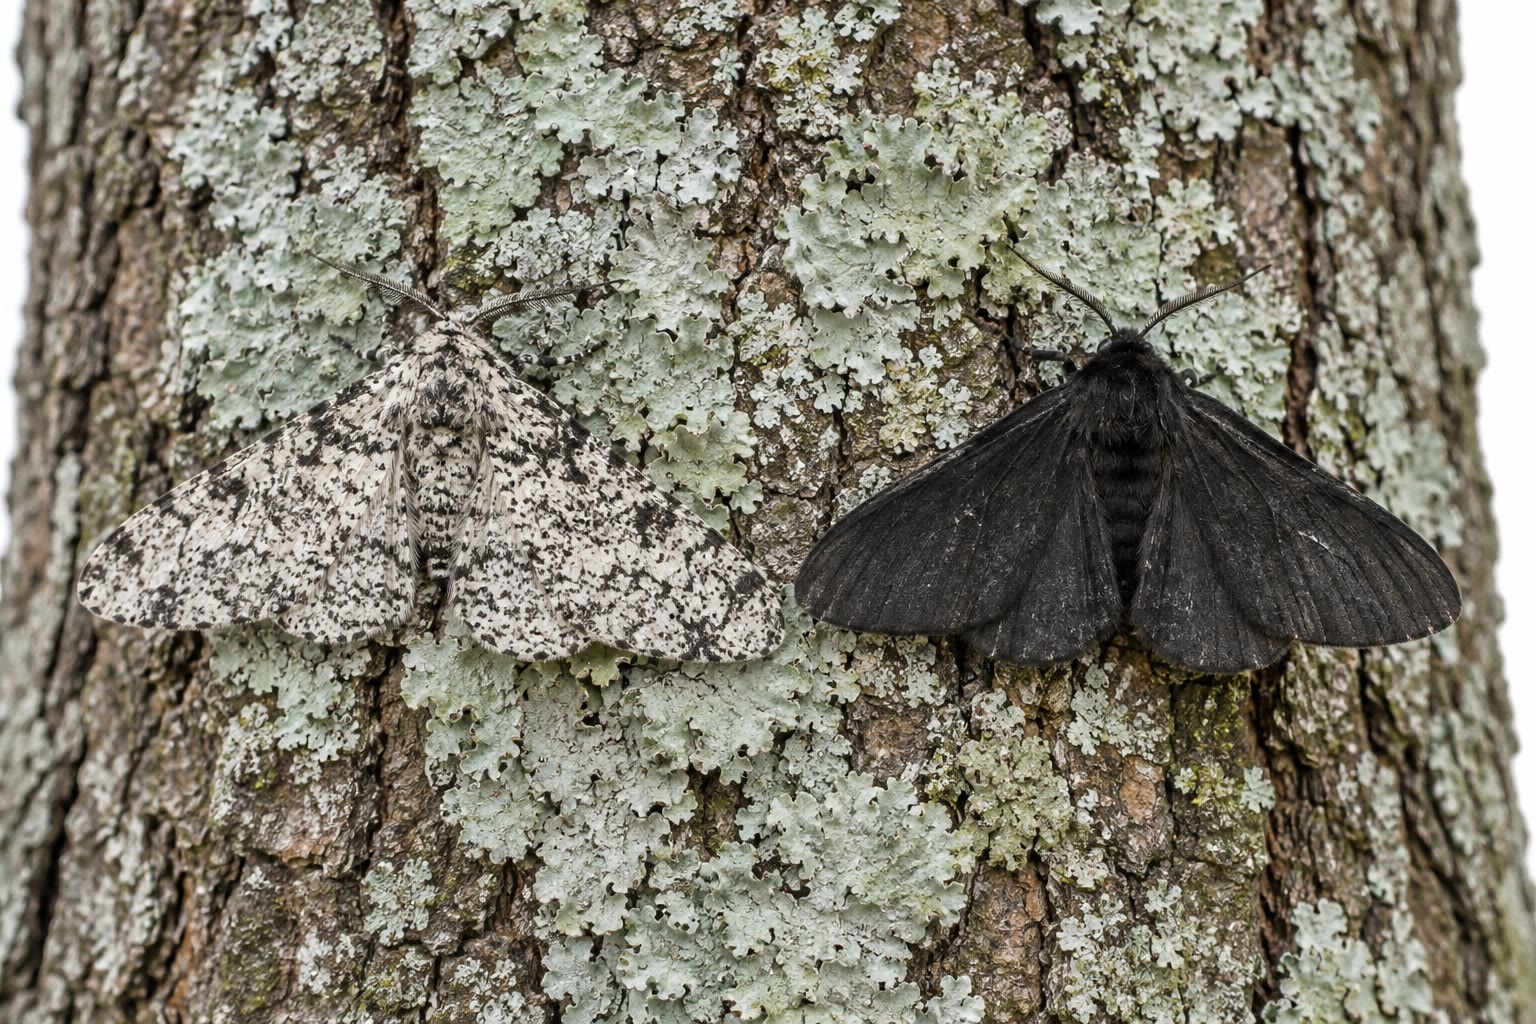
\includegraphics[width=0.46\linewidth]{images/book4/ai/b4-22-peppered-moths.jpg}\hspace{0.04\linewidth}
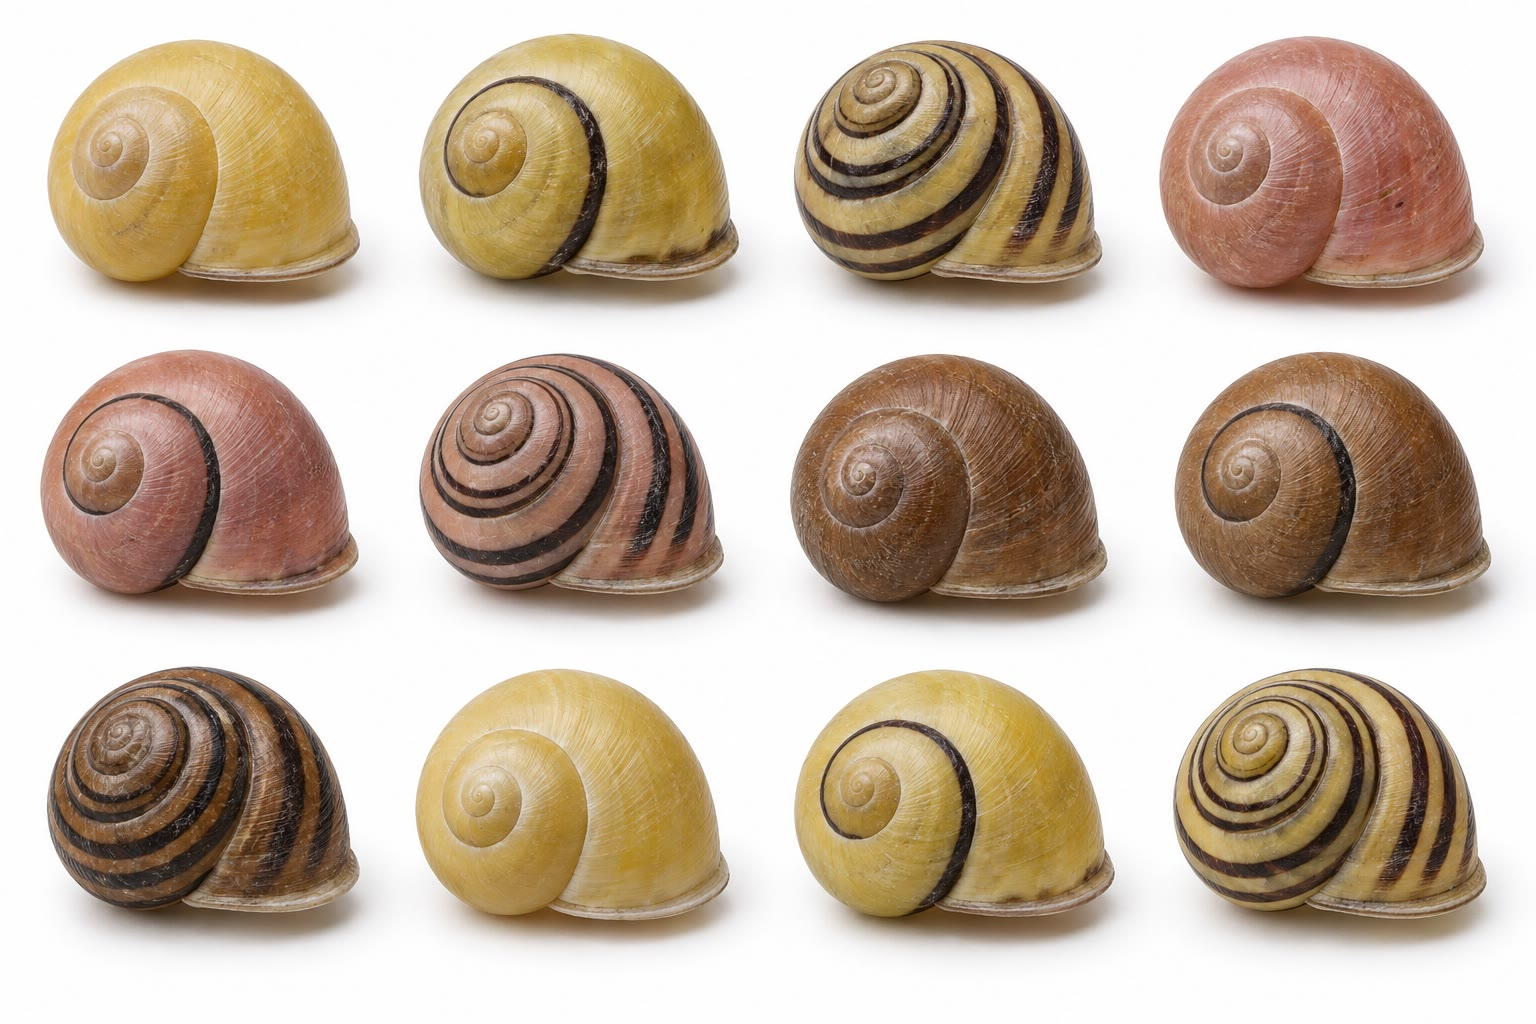
\includegraphics[width=0.46\linewidth]{images/book4/ai/b4-22-banded-snails.jpg}

{\small إلى اليسار: شكلا الفراشة الفلفلية على الأشنة ---
وأيهما يجده الطائر يتوقف على اللحاء. وإلى اليمين: تعدد
أشكال صدفة حلزون البساتين، وألوانه وأشرطته تبقيها في كل
جمهرة مفترسات تتعلم الشكل الشائع.}
\end{omfigure}

\section{تمارين}

\begin{exercise}[$\star$]\label{exo:b2:population-genetics:1}
في عينة من 1000 شخص، 640 منهم $MM$ و320 $MN$ و40 $NN$.
احسب التواترات الأليلية وتوقعات هاردي--واينبرغ.
فهل الجمهرة في توازن؟
\end{exercise}

\begin{exercise}[$\star$]\label{exo:b2:population-genetics:2}
المهق \omterm{def:b2:meiosis-heredity:vocabulary}{متنحٍّ} ويصيب شخصًا من كل \num{20000}.
احسب \omterm{def:b2:population-genetics:frequencies}{التواتر الأليلي} وتواتر الحاملين.
\end{exercise}

\begin{exercise}[$\star$]\label{exo:b2:population-genetics:3}
عرّف \omterm{def:b2:population-genetics:fitness}{اللياقة} \omterm{def:b2:population-genetics:fitness}{ومعامل الانتقاء} \omterm{thm:b2:population-genetics:heritability}{وقابلية التوريث}، وأعطِ
القوى الخمس التي تغير التواترات الأليلية.
\end{exercise}

\begin{exercise}[$\star$]\label{exo:b2:population-genetics:4}
أعطِ مثالًا واحدًا لكل من \omterm{prop:b2:population-genetics:kinds}{الانتقاء الموجّه} والمثبِّت والموازن،
مع عامل الانتقاء في كل منها.
\end{exercise}

\begin{exercise}[$\star\star$]\label{exo:b2:population-genetics:5}
\omterm{def:b2:meiosis-heredity:vocabulary}{أليل} \omterm{def:b2:meiosis-heredity:vocabulary}{متنحٍّ} مميت تواتره $0.02$. فكم جيلًا يلزم
لتنصيفه؟ وكم لبلوغ $0.001$؟ وماذا يقول ذلك عن
أثر منع المصابين من التكاثر؟
\end{exercise}

\begin{exercise}[$\star\star$]\label{exo:b2:population-genetics:6}
عند $w_{AA} = 1$ و$w_{Aa} = 1$ و$w_{aa} = 0.8$ و$p = 0.3$، احسب
$\bar w$ و$p'$ و$\Delta p$. وأعد ذلك عند $p = 0.9$. ولماذا كان
التغير الثاني أصغر بكثير؟
\end{exercise}

\begin{exercise}[$\star\star$]\label{exo:b2:population-genetics:7}
\omterm{def:b2:meiosis-heredity:vocabulary}{لمتماثل اللواقح} المنجلي $w = 0.2$ ولمتماثل اللواقح السوي
$w = 0.88$ في منطقة ملارية، ولمتغايري اللواقح $w = 1$. احسب
التواتر التوازني \omterm{def:b2:meiosis-heredity:vocabulary}{للأليل} المنجلي وكسر
الأطفال المولودين بالمرض عند التوازن.
\end{exercise}

\begin{exercise}[$\star\star$]\label{exo:b2:population-genetics:8}
ينشأ \omterm{def:b2:meiosis-heredity:vocabulary}{متنحٍّ} مميت \omterm{def:b2:genome-diversification:mutation}{بالطفرة} عند $\mu = \qty{2e-5}{}$ لكل
عرس. احسب تواتره التوازني وكسر
المواليد المصابين. ثم لمميت \omterm{def:b2:meiosis-heredity:vocabulary}{سائد} (قبل التكاثر) بالمعدل
نفسه: فأي كسر من المواليد؟
\end{exercise}

\begin{exercise}[$\star\star$]\label{exo:b2:population-genetics:9}
جمهرة من 50 فردًا متكاثرًا تبدأ عند $H = 0.5$.
احسب تغايرها اللاقحي بعد 10 و50 و200 جيل. وكم
يجب أن تكون الجمهرة كبيرة لتبقي \qty{90}{\%} من
تغايرها اللاقحي على مدى 100 جيل؟
\end{exercise}

\begin{exercise}[$\star\star\star$]\label{exo:b2:population-genetics:10}
تستعمر جزيرةً 10 طيور من جمهرة بر رئيس
تواتر \omterm{def:b2:meiosis-heredity:vocabulary}{أليل} فيها $0.1$. احسب احتمال أن
يكون \omterm{def:b2:meiosis-heredity:vocabulary}{الأليل} غائبًا عن المؤسسين، واحتمال أن
يُثبَّت في النهاية على الجزيرة إذا وُجد في نسخة واحدة.
وقارن بالبر الرئيس.
\end{exercise}

\begin{exercise}[$\star\star\star$]\label{exo:b2:population-genetics:11}
لمردود الحليب $h^{2} = 0.3$ وانحراف معياري قدره
\qty{1000}{L}. ويبقي مربٍّ أعلى \qty{20}{\%} من البقرات
أمهات (ومتوسطهن أعلى من متوسط القطيع بمقدار $1.4$ انحراف معياري).
احسب الاستجابة في الجيل. وإن اختيرت الثيران من
أعلى \qty{1}{\%} (بمتوسط أعلى بمقدار $2.7$ انحراف معياري)، فما
الاستجابة؟ ولماذا تبطؤ الاستجابة بعد أجيال كثيرة؟
\end{exercise}

\begin{exercise}[$\star\star\star$]\label{exo:b2:population-genetics:12}
«الانتقاء أعمى عما لا يراه.» ناقش، مستعينًا
\omterm{def:b2:meiosis-heredity:vocabulary}{بالأليل} المتنحي في متغايري اللواقح، وبالطفرة المحايدة، وبالصفة
التي قابلية توريثها صفر، ما الذي يستطيع الانتقاء أن يفعل فيه وما لا
يستطيع.
\end{exercise}

\section{مسألة: الفراشة والجزيرة والقطيع}

\begin{problem}[{مسألة نهاية الأسبوع --- حساب صعود الفراشة
الفلفلية من معادلة الانتقاء، ومتابعة انجراف جمهرة مؤسِّسة
وتزاوجها الداخلي، وإقامة توازن بين الطفرة والانتقاء، و
التنبؤ ببرنامج مربٍّ، وتنتهي إلى معامل انتقاء
الفراشة، وتغاير الجزيرة اللاقحي، وكسب القطيع}]
\label{pb:b2:population-genetics:1}
الفراشة الفلفلية: \omterm{def:b2:meiosis-heredity:vocabulary}{أليل} السواد $M$ \omterm{def:b2:meiosis-heredity:vocabulary}{سائد}، وتواتره $p_0 = 0.001$
سنة 1848؛ و\qty{90}{\%} من الفراشات سوداء بعد 50 جيلًا؛ وافترض
$w_{MM} = w_{Mm} = 1$ و$w_{mm} = 1 - s$. والجزيرة: أسسها 12
طائرًا من بر رئيس فيه $H = 0.4$ \omterm{def:b2:meiosis-heredity:vocabulary}{وأليل} \omterm{def:b2:meiosis-heredity:vocabulary}{متنحٍّ} ضار
تواتره $q = 0.05$؛ وتحمل الجزيرة 40 طائرًا متكاثرًا
بعد ذلك. \omterm{def:b2:genome-diversification:mutation}{والطفرة}: $\mu = \qty{1e-5}{}$. والقطيع: $h^{2} = 0.4$،
وانحراف معياري \qty{800}{L}.

\medskip
\noindent\textbf{الجزء الأول --- الفراشة.}
\begin{enumerate}
  \item في سنة 1848، أي كسر من الفراشات كان أسود، وأي
        كسر من أليلات $M$ كان يجلس في متغايري اللواقح؟
  \item بيّن أنه، مع سيادة $M$، يخضع تواتر \omterm{def:b2:meiosis-heredity:vocabulary}{الأليل}
        الفاتح للعلاقة $q' = q(1 - sq)/(1 - sq^{2})$.
  \item انطلاقًا من $q_0 = 0.999$، احسب $q$ بعد جيل واحد
        عند $s = 0.3$.
  \item كون \qty{90}{\%} سوداء يعني $q^{2} = 0.1$. فما $q$ حينئذ؟
  \item بالتجريب على العلاقة التراجعية (أو بالتقريب
        $\Delta q \approx -sq^{2}p$ ما دام $q$ قريبًا من 1)، قدّر
        عدد الأجيال اللازم عند $s = 0.3$ لنقل $q$ من $0.999$
        إلى $0.32$، وقارنه بالقيمة 50 الملحوظة.
  \item بعد قوانين الهواء النظيف تصير الأفضلية للشكل الفاتح، فيصير $s
        = 0.3$ ضد $mm$ هو $s = 0.3$ ضد $M\_$. بيّن
        أن $\Delta p = -spq^{2}/\bar w$، وفسّر لماذا تكون عودة
        الشكل الفاتح بطيئة في البداية وتنتهي بهبوط
        أسّي \omterm{def:b2:meiosis-heredity:vocabulary}{للأليل} $M$، في حين بدأ الصعود أسّيًا
        وانتهى زحفًا.
\end{enumerate}

\medskip
\noindent\textbf{الجزء الثاني --- الجزيرة.}
\begin{enumerate}[resume]
  \item احسب احتمال ألا يحمل أحد من المؤسسين الاثني عشر
        الأليلَ الضار.
  \item احسب التغاير اللاقحي المنتظر بعد جيل
        التأسيس (مسحوبًا من $H = 0.4$ بواسطة 12 فردًا، أي 24
        نسخة مورّثية).
  \item احسب التغاير اللاقحي بعد 100 جيل عند $N =
        40$، كسرًا من تغاير البر الرئيس.
  \item تظهر \omterm{def:b2:genome-diversification:mutation}{طفرة} محايدة في طائر واحد. احسب
        احتمال تثبيتها والزمن المنتظر للتثبيت إن
        ثُبِّتت.
  \item تتزاوج طيور الجزيرة عشوائيًا لكنها كلها قريبة. وإذ
        يتراكم $F = 1/(2N)$ في الجيل ليبلغ نحو $0.3$ بعد
        30 جيلًا، احسب تواتر متماثلي اللواقح المصابين
        \omterm{def:b2:meiosis-heredity:vocabulary}{للأليل} عند $q = 0.05$، مع \omterm{prop:b2:population-genetics:inbreeding}{التزاوج الداخلي} ودونه.
  \item يصل طائر واحد من البر الرئيس في كل جيل. فسّر ماذا
        يفعل ذلك بتباعد الجزيرة وبحملها.
\end{enumerate}

\medskip
\noindent\textbf{الجزء الثالث --- التوازن.}
\begin{enumerate}[resume]
  \item احسب التواتر التوازني \omterm{def:b2:meiosis-heredity:vocabulary}{لمتنحٍّ} مميت تغذيه
        $\mu = 10^{-5}$، وكسر المواليد المصابين.
  \item احسب الأمر نفسه عند $s = 0.1$ (أي \omterm{def:b2:meiosis-heredity:vocabulary}{متنحٍّ} ضار
        ضررًا خفيفًا).
  \item احسب التوازن \omterm{def:b2:meiosis-heredity:vocabulary}{لأليل} \omterm{def:b2:meiosis-heredity:vocabulary}{سائد} ضرره عند
        تغاير اللواقح $hs = 0.05$.
  \item يشفي الطب المميت فيهبط $s$ إلى $0.1$. فكيف
        يتغير التوازن، وكم تستغرق الجمهرة (برتبة
        المقدار) لتبلغه؟
  \item في المورثوم \num{20000} مورّثة تطفر كل منها إلى
        \omterm{def:b2:meiosis-heredity:vocabulary}{متنحٍّ} مميت بمعدل $10^{-5}$. فكم أليلًا مميتًا يحمل
        الشخص الوسطي في حالة تغاير اللواقح؟ (فعند
        التوازن يكون لكل موقع $2\hat q$ نسخة في الشخص.)
  \item فسّر لماذا يوافق ذلك العدد جمهرةً صحيحة ولماذا
        يجعل زواج أبناء العم مكلفًا.
\end{enumerate}

\medskip
\noindent\textbf{الجزء الرابع --- القطيع.}
\begin{enumerate}[resume]
  \item يبقي المربّي أعلى \qty{30}{\%} من البقرات (بمتوسط $1.16$
        انحراف معياري فوق القطيع). احسب فرق
        الانتقاء باللترات والاستجابة.
  \item بعد خمسة أجيال من الانتقاء نفسه، ما الكسب
        المنتظر، ولماذا قد يكون الكسب الحقيقي أصغر؟
  \item تسهم الثيران بنصف المورّثات وتُنتقى من أعلى
        \qty{2}{\%} ($2.4$ انحراف معياري). احسب الاستجابة
        حين تُنتقى البقرات والثيران كما ذُكر (بمتوسط الفرقين).
  \item قطيع كل بقراته مستنسخات من حيوان واحد: فما
        $h^{2}$ وما الاستجابة؟ وماذا يقول ذلك عن
        \omterm{thm:b2:population-genetics:heritability}{قابلية التوريث}؟
  \item لجمهرة عصافير $h^{2} = 0.7$ لعمق المنقار ويترك
        الجفاف ناجين أعمق بمقدار \qty{0.6}{mm}. تنبّأ
        بالجيل التالي.
  \item يتحول المربّي إلى صفة لها $h^{2} = 0.1$. فأي
        فرق انتقاء، بالانحرافات المعيارية، يعطي
        الاستجابة نفسها التي في السؤال 19؟
  \item اذكر النتيجة: معامل انتقاء الفراشة $s$ وزمن بلوغ \qty{90}{\%}
        سوادًا، وتغاير الجزيرة اللاقحي بعد 100 جيل،
        واستجابة القطيع في الجيل.
\end{enumerate}
\end{problem}
